% This is the University of Chicago Graham School Master of Science in Analytics
% template. Much of it is based on the Reed College LaTeX thesis template.
% Most of the work for the Reec College template was done by Sam Noble (SN),
% Later comments etc. by Ben Salzberg (BTS).
% Additional restructuring and APA support by Jess Youngberg (JY).
% Justin M. Shea (JMS) built on their good open source work.
% Your comments and suggestions are more than welcome:
% please email, them to justinshea@uchicago.edu.
%
% Any line that starts with a percent symbol is a comment.
% They won't show up in the document, and are useful for notes
% to yourself and explaining commands.
% Commenting also removes a line from the document;
% very handy for troubleshooting problems. -BTS
%%
%% Preamble
%%
% \documentclass{<something>} must begin each LaTeX document
% Added by JMS
\documentclass[12pt,oneside]{chicagocapstone}
% END of JMS add
% Packages are extensions to the basic LaTeX functions. Whatever you
% want to typeset, there is probably a package out there for it.
% Check out CTAN to see: http://www.ctan.org/
%%
\usepackage{graphicx,latexsym}
\usepackage{amsmath}
\usepackage{amssymb,amsthm}
\usepackage{longtable,booktabs,setspace}
\usepackage[hyphens]{url}
% Added by CII
\usepackage{hyperref}
\usepackage{lmodern}
\usepackage{float}
\floatplacement{figure}{H}
% End of CII addition
\usepackage{rotating}


% Added by CII (Thanks, Hadley!)
% Use ref for internal links
\renewcommand{\hyperref}[2][???]{\autoref{#1}}
\def\chapterautorefname{Chapter}
\def\sectionautorefname{Section}
\def\subsectionautorefname{Subsection}
% End of CII addition

% Added by CII
\usepackage{caption}
\captionsetup{width=5in}
% End of CII addition

% Added by JMS
\usepackage{mathptmx} % Times New Roman fonts
% End of add by JMS

% Syntax highlighting #22
  \usepackage{color}
  \usepackage{fancyvrb}
  \newcommand{\VerbBar}{|}
  \newcommand{\VERB}{\Verb[commandchars=\\\{\}]}
  \DefineVerbatimEnvironment{Highlighting}{Verbatim}{commandchars=\\\{\}}
  % Add ',fontsize=\small' for more characters per line
  \usepackage{framed}
  \definecolor{shadecolor}{RGB}{248,248,248}
  \newenvironment{Shaded}{\begin{snugshade}}{\end{snugshade}}
  \newcommand{\AlertTok}[1]{\textcolor[rgb]{0.94,0.16,0.16}{#1}}
  \newcommand{\AnnotationTok}[1]{\textcolor[rgb]{0.56,0.35,0.01}{\textbf{\textit{#1}}}}
  \newcommand{\AttributeTok}[1]{\textcolor[rgb]{0.77,0.63,0.00}{#1}}
  \newcommand{\BaseNTok}[1]{\textcolor[rgb]{0.00,0.00,0.81}{#1}}
  \newcommand{\BuiltInTok}[1]{#1}
  \newcommand{\CharTok}[1]{\textcolor[rgb]{0.31,0.60,0.02}{#1}}
  \newcommand{\CommentTok}[1]{\textcolor[rgb]{0.56,0.35,0.01}{\textit{#1}}}
  \newcommand{\CommentVarTok}[1]{\textcolor[rgb]{0.56,0.35,0.01}{\textbf{\textit{#1}}}}
  \newcommand{\ConstantTok}[1]{\textcolor[rgb]{0.00,0.00,0.00}{#1}}
  \newcommand{\ControlFlowTok}[1]{\textcolor[rgb]{0.13,0.29,0.53}{\textbf{#1}}}
  \newcommand{\DataTypeTok}[1]{\textcolor[rgb]{0.13,0.29,0.53}{#1}}
  \newcommand{\DecValTok}[1]{\textcolor[rgb]{0.00,0.00,0.81}{#1}}
  \newcommand{\DocumentationTok}[1]{\textcolor[rgb]{0.56,0.35,0.01}{\textbf{\textit{#1}}}}
  \newcommand{\ErrorTok}[1]{\textcolor[rgb]{0.64,0.00,0.00}{\textbf{#1}}}
  \newcommand{\ExtensionTok}[1]{#1}
  \newcommand{\FloatTok}[1]{\textcolor[rgb]{0.00,0.00,0.81}{#1}}
  \newcommand{\FunctionTok}[1]{\textcolor[rgb]{0.00,0.00,0.00}{#1}}
  \newcommand{\ImportTok}[1]{#1}
  \newcommand{\InformationTok}[1]{\textcolor[rgb]{0.56,0.35,0.01}{\textbf{\textit{#1}}}}
  \newcommand{\KeywordTok}[1]{\textcolor[rgb]{0.13,0.29,0.53}{\textbf{#1}}}
  \newcommand{\NormalTok}[1]{#1}
  \newcommand{\OperatorTok}[1]{\textcolor[rgb]{0.81,0.36,0.00}{\textbf{#1}}}
  \newcommand{\OtherTok}[1]{\textcolor[rgb]{0.56,0.35,0.01}{#1}}
  \newcommand{\PreprocessorTok}[1]{\textcolor[rgb]{0.56,0.35,0.01}{\textit{#1}}}
  \newcommand{\RegionMarkerTok}[1]{#1}
  \newcommand{\SpecialCharTok}[1]{\textcolor[rgb]{0.00,0.00,0.00}{#1}}
  \newcommand{\SpecialStringTok}[1]{\textcolor[rgb]{0.31,0.60,0.02}{#1}}
  \newcommand{\StringTok}[1]{\textcolor[rgb]{0.31,0.60,0.02}{#1}}
  \newcommand{\VariableTok}[1]{\textcolor[rgb]{0.00,0.00,0.00}{#1}}
  \newcommand{\VerbatimStringTok}[1]{\textcolor[rgb]{0.31,0.60,0.02}{#1}}
  \newcommand{\WarningTok}[1]{\textcolor[rgb]{0.56,0.35,0.01}{\textbf{\textit{#1}}}}

% To pass between YAML and LaTeX the dollar signs are added by CII
\title{Music Generator}
\author{Terry Wang, Rima Mittal, Joshua Goldberg}
\date{March, 2020} % The month and year that you submit your FINAL draft)
\division{Graham School}
\advisor{Yuri Balasanov}
\institution{University of Chicago}
\degree{Master of Science in Analytics}
% End of CII addition

\department{Continuing Liberal and Professional Studies}

% Added by CII
%%% Copied from knitr
%% maxwidth is the original width if it's less than linewidth
%% otherwise use linewidth (to make sure the graphics do not exceed the margin)
\makeatletter
\def\maxwidth{ %
  \ifdim\Gin@nat@width>\linewidth
    \linewidth
  \else
    \Gin@nat@width
  \fi
}
\makeatother

\renewcommand{\contentsname}{Table of Contents}
% End of CII addition

\setlength{\parskip}{0pt}

% Added by CII
  %\setlength{\parskip}{\baselineskip}
  \usepackage[parfill]{parskip}

\providecommand{\tightlist}{%
  \setlength{\itemsep}{0pt}\setlength{\parskip}{0pt}}


\Abstract{
Maximum 40 to 50 words. An abstract is a concise description of your project. It should include very brief description of the problem, purpose, method, key results, and conclusions. Note you may want to write the abstract after writing the report.

\bigskip 
\bigskip
\bigskip

\textbf{Keywords}: Include 6 to 10 keywords on the same page as the abstract. Select keywords that would help a researcher retrieve your report.

\bigskip 
\bigskip
\bigskip

\textbf{NOTE:} Do not use ``\#'' or ``\#\#'' symbols to start new sections in the abstract section, as one typically would in other r markdown documents. Doing so will result in generating a table of contents entry \emph{prior} to the Introduction, which is not desirable.
}

% Added by JMS
\Executive{
The executive summary is a maximum one page, double spaced summary of your report aimed at informing someone, who does not read the entire report, about your project. The executive summary is an extended version of the abstract with more space allocated to the key findings of the project and the conclusions and recommendations. You may want to write this section after writing the report.

Second Paragraph.

Third Paragraph.

\bigskip
\bigskip
\bigskip

\textbf{NOTE:} Like the abstract, do not use ``\#'' or ``\#\#'' symbols to start new sections in the executive summary section. Doing so will result in generating a table table of contents entry \emph{prior} to the Introduction, which is not desirable.
}
% End of JMS add

\Acknowledgements{

}

\Dedication{

}

\Preface{

}


% End of CII addition
%%
%% End Preamble
%%
%
\begin{document}

% Everything below added by CII
  \maketitle

\frontmatter % this stuff will be roman-numbered
\pagestyle{empty} % this removes page numbers from the frontmatter


%% Reorganized by JMS
  \begin{abstract}
    Maximum 40 to 50 words. An abstract is a concise description of your project. It should include very brief description of the problem, purpose, method, key results, and conclusions. Note you may want to write the abstract after writing the report.
    
    \bigskip 
    \bigskip
    \bigskip
    
    \textbf{Keywords}: Include 6 to 10 keywords on the same page as the abstract. Select keywords that would help a researcher retrieve your report.
    
    \bigskip 
    \bigskip
    \bigskip
    
    \textbf{NOTE:} Do not use ``\#'' or ``\#\#'' symbols to start new sections in the abstract section, as one typically would in other r markdown documents. Doing so will result in generating a table of contents entry \emph{prior} to the Introduction, which is not desirable.
  \end{abstract}
 % Added by JMS
  \begin{executive}
    The executive summary is a maximum one page, double spaced summary of your report aimed at informing someone, who does not read the entire report, about your project. The executive summary is an extended version of the abstract with more space allocated to the key findings of the project and the conclusions and recommendations. You may want to write this section after writing the report.
    
    Second Paragraph.
    
    Third Paragraph.
    
    \bigskip
    \bigskip
    \bigskip
    
    \textbf{NOTE:} Like the abstract, do not use ``\#'' or ``\#\#'' symbols to start new sections in the executive summary section. Doing so will result in generating a table table of contents entry \emph{prior} to the Introduction, which is not desirable.
  \end{executive}
 % End of JMS




  \hypersetup{linkcolor=black}
  \setcounter{tocdepth}{2}
  \tableofcontents

  \listoffigures

  \listoftables

%% END of Reorganization by JMS

\mainmatter % here the regular arabic numbering starts
\pagestyle{fancyplain} % turns page numbering back on

\hypertarget{introduction}{%
\chapter*{Introduction}\label{introduction}}
\addcontentsline{toc}{chapter}{Introduction}

We built a deep learning model to help individuals generate interesting music ideas. The model is a GAN-based generator. The data used to train the generator are 130,000 midi files across many different genres of music.

\hypertarget{problem-statement}{%
\section*{Problem Statement}\label{problem-statement}}
\addcontentsline{toc}{section}{Problem Statement}

In 1950s, experimental music composers wrote music using randomized statistical modelling. In 1990s, David Bowie built the Verbasizer, which implemented a random re-ordering of group of words and sentences to produce potentially significant lyrical combinations. Nowadays, there is an entire industry built around AI generated music including Flow Machines, IBM Watson Beat and Google's NSynth.

Our purpose is to build an effective platform to help artists in their creative process and assist them in music composition. Note that artists do not have to be professionally designated. Any individual interested in creating music should find the platform useful and empowering. The first concrete step we need to take to achieve that goal is to build a music generation model that is able to generate music that is similar to what a human would compose in the style of music the model is trained on.

\hypertarget{research-purpose}{%
\section*{Research Purpose}\label{research-purpose}}
\addcontentsline{toc}{section}{Research Purpose}

The purpose of this project is to develop a deep learning based music generator (instrumental music) which has a good understanding of the language of music and is able to generate human-like outputs, ultimately helping musicians and non-musicians alike to develop and refine musical ideas, and facilitate them in the music composition process. We divided the project into two parts, Generation and Validation.

By doing this iteratively, the weights and parameters of the model will hopefully converge to a point at which the music generated is satisfactory to the user, who can use the output of the model, or save the weights for future use. In a sense, we are democratizing deep learning to non-technical users wishing to generate new music ideas in a novel way. Moreover, we expect the algorithmic process to able to explore more music combinations than any individual, and thus provide a more holistic and creative approach to music creation.

\hypertarget{variables-and-scope}{%
\section*{Variables and Scope}\label{variables-and-scope}}
\addcontentsline{toc}{section}{Variables and Scope}

Our data consists of 130,000 midi files curated by a Reddit user, with a size of 3.65GB uncompressed. The collection has a great amount of variety representing all major genres in classical, jazz, metal, pop, etc. These midi files can be parsed by python packages such as midi and music21 into numpy arrays that preserves the note duration information, and our model will be trained on them.

\hypertarget{writing-tips}{%
\section*{Writing Tips}\label{writing-tips}}
\addcontentsline{toc}{section}{Writing Tips}
\begin{itemize}
\tightlist
\item
  Develop an outline of what you are going to write for each section before you start writing
\item
  Good writing follows a general format: introduction, body, and conclusion. This rule applies to the entire project, to each section, and to each paragraph
\item
  Each paragraph presents only one idea and follows the \textbf{MEAL} rule
  \begin{itemize}
  \tightlist
  \item
    \textbf{M}ain: start the paragraph with the \emph{Main} idea
  \item
    \textbf{E}xplain the concepts and define the terms
  \item
    \textbf{A}nalyze the idea
  \item
    \textbf{L}ink: conclude the paragraph and \emph{Link} it to the next paragraph
  \end{itemize}
\item
  Make sure to define any concepts or terms that reader might be unfamiliar with right before or after they are used
\end{itemize}
\textbf{More info}

And here's some other random info: the first paragraph after a chapter title or section head \emph{shouldn't be} indented, because indents are to tell the reader that you're starting a new paragraph. Since that's obvious after a chapter or section title, proper typesetting doesn't add an indent there.

\textbf{Spacing and Markdown}

Be careful with your spacing in \emph{Markdown} documents. While white-space largely is ignored, it does at times give \emph{Markdown} signals as to how to proceed. As a habit, try to keep everything left aligned whenever possible, especially as you type a new paragraph. In other words, there is no need to indent basic text in the Rmd document (in fact, it might cause your text to do funny things if you do).

\hypertarget{rmd-basics}{%
\section*{R Markdown Basics}\label{rmd-basics}}
\addcontentsline{toc}{section}{R Markdown Basics}

\hypertarget{lists}{%
\subsection*{Lists}\label{lists}}
\addcontentsline{toc}{subsection}{Lists}

It's easy to create a list. It can be unordered like
\begin{itemize}
\tightlist
\item
  Item 1
\item
  Item 2
\end{itemize}
or it can be ordered like
\begin{enumerate}
\def\labelenumi{\arabic{enumi}.}
\tightlist
\item
  Item 1
\item
  Item 2
\end{enumerate}
Notice that I intentionally mislabeled Item 2 as number 4. \emph{Markdown} automatically figures this out! You can put any numbers in the list and it will create the list. Check it out below.

To create a sub-list, just indent the values a bit (at least four spaces or a tab). (Here's one case where indentation is key!)
\begin{enumerate}
\def\labelenumi{\arabic{enumi}.}
\tightlist
\item
  Item 1
\item
  Item 2
\item
  Item 3
  \begin{itemize}
  \tightlist
  \item
    Item 3a
  \item
    Item 3b
  \end{itemize}
\end{enumerate}
\hypertarget{line-breaks}{%
\subsection*{Line breaks}\label{line-breaks}}
\addcontentsline{toc}{subsection}{Line breaks}

Make sure to add white space between lines if you'd like to start a new paragraph. Look at what happens below in the outputted document if you don't:

Here is the first sentence. Here is another sentence. Here is the last sentence to end the paragraph.
This should be a new paragraph.

\emph{Now for the correct way:}

Here is the first sentence. Here is another sentence. Here is the last sentence to end the paragraph.

This should be a new paragraph.

\hypertarget{background}{%
\chapter*{Background}\label{background}}
\addcontentsline{toc}{chapter}{Background}

This section provides a literature review that informs the reader in the following ways:
\begin{itemize}
\tightlist
\item
  Provides background information so the reader may understand related concepts
\item
  Identifies and defines concepts and variables involved and ummarizes what is known
\item
  Motivates the research and highlights its importance within the literature described
\end{itemize}
\textbf{Introduction}
\begin{itemize}
\tightlist
\item
  Define the focus: e.g., pricing models based on emerging market conditions
\item
  Introduce the thesis: e.g., existing models are ex-post and there is a need for ex-ante
\end{itemize}
\textbf{Body}
\begin{itemize}
\tightlist
\item
  Elaborate on the thesis
\item
  Review literature to substantiate your assumptions and build support for the thesis
\item
  Resolve conflicting findings to the thesis and formulate alternative theses
\item
  Discuss why the alternatives are not favored and Identify knowledge gaps
\item
  Identify and motivate the contribution of the research
\end{itemize}
\textbf{Conclusion}
\begin{itemize}
\tightlist
\item
  Summarize the evidence in support of your thesis
\item
  Summarize why alternative theses are not favored
\item
  State the research question and hypotheses
\end{itemize}
\newpage

\hypertarget{code-chunks}{%
\subsection*{Code chunks}\label{code-chunks}}
\addcontentsline{toc}{subsection}{Code chunks}

When you click the \textbf{Knit} button above a document will be generated that includes both content as well as the output of any embedded code chunks within the document. You can embed a code chunk as demonstrated below.

The \texttt{sleep} data is a built-in \textbf{R} dataset (\texttt{Student-t} (1908) \emph{The probable error of the mean}. Biometrika, 6, 20). It shows the effect of two soporific drugs (increase in hours of sleep compared to control) on 10 patients.

Use the \texttt{kable} function to create quick, decent looking tables. Other packages for higher quality tables are \href{https://cran.r-project.org/web/packages/xtable/index.html}{xtable} and \href{https://cran.r-project.org/web/packages/stargazer/index.html}{stargazar}. These are especially recommended for working with \LaTeX~output.
\begin{Shaded}
\begin{Highlighting}[]
\KeywordTok{data}\NormalTok{(sleep)}
\NormalTok{sleep2 <-}\StringTok{ }\KeywordTok{data.frame}\NormalTok{(sleep[}\DecValTok{1}\OperatorTok{:}\DecValTok{10}\NormalTok{, }\DecValTok{1}\NormalTok{], sleep[}\DecValTok{11}\OperatorTok{:}\DecValTok{20}\NormalTok{, }\DecValTok{1}\NormalTok{])}
\KeywordTok{colnames}\NormalTok{(sleep2) <-}\StringTok{ }\KeywordTok{c}\NormalTok{(}\StringTok{"extra_sleep_drug1"}\NormalTok{, }\StringTok{"extra_sleep_drug2"}\NormalTok{)}
\KeywordTok{kable}\NormalTok{(sleep2, }\DataTypeTok{row.names =} \OtherTok{TRUE}\NormalTok{, }\DataTypeTok{caption =} \StringTok{"Sleep Data"}\NormalTok{, }
              \DataTypeTok{format =} \StringTok{"latex"}\NormalTok{, }\DataTypeTok{longtable =} \OtherTok{TRUE}\NormalTok{)}
\end{Highlighting}
\end{Shaded}
\begin{longtable}[t]{l|r|r}
\caption{\label{tab:sleep}Sleep Data}\\
\hline
  & extra\_sleep\_drug1 & extra\_sleep\_drug2\\
\hline
1 & 0.7 & 1.9\\
\hline
2 & -1.6 & 0.8\\
\hline
3 & -0.2 & 1.1\\
\hline
4 & -1.2 & 0.1\\
\hline
5 & -0.1 & -0.1\\
\hline
6 & 3.4 & 4.4\\
\hline
7 & 3.7 & 5.5\\
\hline
8 & 0.8 & 1.6\\
\hline
9 & 0.0 & 4.6\\
\hline
10 & 2.0 & 3.4\\
\hline
\end{longtable}
\hypertarget{linked-tables-and-list-of-tables}{%
\subsection*{Linked tables and List of Tables}\label{linked-tables-and-list-of-tables}}
\addcontentsline{toc}{subsection}{Linked tables and List of Tables}

We linked Table \ref{tab:sleep} above to the \texttt{List\ of\ Tables} section following the table of contents. For this to work properly, two steps are required.
\begin{enumerate}
\def\labelenumi{\arabic{enumi}.}
\tightlist
\item
  The code chunk of the table must be given a label argument. ie; \texttt{\{r\ sleep,\ args\}}.
\item
  Define a caption in the \texttt{kable} function (\texttt{caption\ =\ "Sleep\ Data"}) call. The caption will be passed to the \textbf{\texttt{List\ of\ Tables}} section and is required for an entry to appear.
\end{enumerate}
\hypertarget{more-than-r-other-languages}{%
\subsection*{More than R: Other Languages}\label{more-than-r-other-languages}}
\addcontentsline{toc}{subsection}{More than R: Other Languages}

R Markdown supports the following languages:
\begin{Shaded}
\begin{Highlighting}[]
\KeywordTok{names}\NormalTok{(knitr}\OperatorTok{::}\NormalTok{knit_engines}\OperatorTok{$}\KeywordTok{get}\NormalTok{())}
\end{Highlighting}
\end{Shaded}
\begin{verbatim}
 [1] "awk"         "bash"        "coffee"      "gawk"        "groovy"     
 [6] "haskell"     "lein"        "mysql"       "node"        "octave"     
[11] "perl"        "psql"        "Rscript"     "ruby"        "sas"        
[16] "scala"       "sed"         "sh"          "stata"       "zsh"        
[21] "highlight"   "Rcpp"        "tikz"        "dot"         "c"          
[26] "fortran"     "fortran95"   "asy"         "cat"         "asis"       
[31] "stan"        "block"       "block2"      "js"          "css"        
[36] "sql"         "go"          "python"      "julia"       "sass"       
[41] "scss"        "theorem"     "lemma"       "corollary"   "proposition"
[46] "conjecture"  "definition"  "example"     "exercise"    "proof"      
[51] "remark"      "solution"   
\end{verbatim}
Of these, if you use \textbf{\texttt{python}}, first load \texttt{reticulate}.
\begin{Shaded}
\begin{Highlighting}[]
\KeywordTok{library}\NormalTok{(reticulate)}
\NormalTok{pyPath <-}\StringTok{ }\KeywordTok{py_discover_config}\NormalTok{()}
\KeywordTok{use_python}\NormalTok{(pyPath}\OperatorTok{$}\NormalTok{python_versions[}\DecValTok{1}\NormalTok{])}
\end{Highlighting}
\end{Shaded}
Create a \texttt{conda} environment to store packages, install, and load one.
\begin{Shaded}
\begin{Highlighting}[]
\KeywordTok{conda_create}\NormalTok{(}\StringTok{"r-reticulate"}\NormalTok{)}
\KeywordTok{py_install}\NormalTok{(}\StringTok{"numpy"}\NormalTok{)}
\NormalTok{numpy <-}\StringTok{ }\KeywordTok{import}\NormalTok{(}\StringTok{"numpy"}\NormalTok{)}
\end{Highlighting}
\end{Shaded}
Define a python code chunk with arguments and run code: \texttt{\{python,\ eval=FALSE,\ etc\}}
\begin{Shaded}
\begin{Highlighting}[]
\ImportTok{import}\NormalTok{ numpy }\ImportTok{as}\NormalTok{ np}
\BuiltInTok{print}\NormalTok{(np.reshape(np.arange(}\DecValTok{1}\NormalTok{,}\DecValTok{25}\NormalTok{), (}\DecValTok{4}\NormalTok{,}\DecValTok{3}\NormalTok{,}\DecValTok{2}\NormalTok{), }\StringTok{"F"}\NormalTok{))}
\end{Highlighting}
\end{Shaded}
Please see the \href{https://rstudio.github.io/reticulate/}{Reticulate: R interface to Python} for more specifics.

Let's not forget about C++/Rcpp enables compilation of C++ into R functions.
\begin{Shaded}
\begin{Highlighting}[]
\PreprocessorTok{#include }\ImportTok{<Rcpp.h>}
\KeywordTok{using} \KeywordTok{namespace}\NormalTok{ Rcpp;}
\CommentTok{// [[Rcpp::export]]}
\NormalTok{NumericVector humanPercent(NumericVector x) \{}
  \ControlFlowTok{return}\NormalTok{ x * }\DecValTok{100}\NormalTok{;}
\NormalTok{\}}
\end{Highlighting}
\end{Shaded}
\begin{Shaded}
\begin{Highlighting}[]
\KeywordTok{humanPercent}\NormalTok{(}\DataTypeTok{x=}\FloatTok{0.0274}\NormalTok{)}
\end{Highlighting}
\end{Shaded}
Please see \href{http://www.rcpp.org/}{Rcpp for Seamless R and C++ Integration}, which is a very mature project and provides many examples.

\newpage

\hypertarget{pressure-plot}{%
\subsection*{Including plots}\label{pressure-plot}}
\addcontentsline{toc}{subsection}{Including plots}

You can also embed plots. For example, here is a way to use the base \textbf{R} graphics package to produce a plot using the built-in \texttt{pressure} dataset. In this case, the \textbf{\texttt{echo=FALSE}} parameter was added to the code chunk to prevent printing the code.
\begin{figure}
\centering
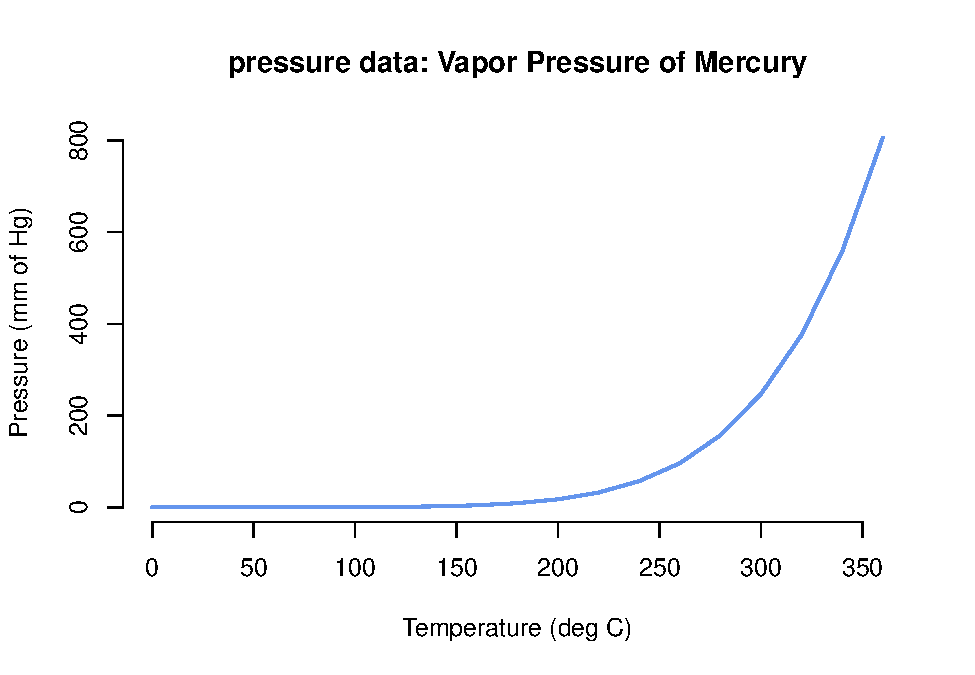
\includegraphics{UChicago-MScA-Capstone_files/figure-latex/pressureplot-1.pdf}
\caption{\label{fig:pressureplot}Pressure Plot}
\end{figure}
This is Figure \ref{fig:pressureplot}: pressure data. Internally, we also labeled the code chunk \texttt{pressureplot} so we can call its contents and print them in the Appendix. see Appendix for the code that generated this plot. There are many arguments which govern the behavior of your code chunks. The creator of \texttt{knitr} has a many notes on this \url{http://yihui.name/knitr/options/}.

\newpage

\hypertarget{ref-labels}{%
\subsection*{R Markdown Tables, Graphics, References, and Labels}\label{ref-labels}}
\addcontentsline{toc}{subsection}{R Markdown Tables, Graphics, References, and Labels}

In addition to the tables that can be automatically generated from a data frame in \textbf{R} that you saw in \protect\hyperlink{rmd-basics}{R Markdown Basics} using the \texttt{kable} function, you can also create tables using \emph{pandoc}. (More information is available at \url{http://pandoc.org/README.html\#tables}.) This might be useful if you don't have values specifically stored in \textbf{R}, but you'd like to display them in table form. Below is an example. Pay careful attention to the alignment in the table and hyphens to create the rows and columns.
\begin{longtable}[]{@{}ccc@{}}
\caption{\label{tab:inher} Correlation of Inheritance Factors for Parents and Child}\tabularnewline
\toprule
\begin{minipage}[b]{0.29\columnwidth}\centering
Factors\strut
\end{minipage} & \begin{minipage}[b]{0.46\columnwidth}\centering
Correlation between Parents \& Child\strut
\end{minipage} & \begin{minipage}[b]{0.16\columnwidth}\centering
Inherited\strut
\end{minipage}\tabularnewline
\midrule
\endfirsthead
\toprule
\begin{minipage}[b]{0.29\columnwidth}\centering
Factors\strut
\end{minipage} & \begin{minipage}[b]{0.46\columnwidth}\centering
Correlation between Parents \& Child\strut
\end{minipage} & \begin{minipage}[b]{0.16\columnwidth}\centering
Inherited\strut
\end{minipage}\tabularnewline
\midrule
\endhead
\begin{minipage}[t]{0.29\columnwidth}\centering
Education\strut
\end{minipage} & \begin{minipage}[t]{0.46\columnwidth}\centering
-0.49\strut
\end{minipage} & \begin{minipage}[t]{0.16\columnwidth}\centering
Yes\strut
\end{minipage}\tabularnewline
\begin{minipage}[t]{0.29\columnwidth}\centering
Socio-Economic Status\strut
\end{minipage} & \begin{minipage}[t]{0.46\columnwidth}\centering
0.28\strut
\end{minipage} & \begin{minipage}[t]{0.16\columnwidth}\centering
Slight\strut
\end{minipage}\tabularnewline
\begin{minipage}[t]{0.29\columnwidth}\centering
Income\strut
\end{minipage} & \begin{minipage}[t]{0.46\columnwidth}\centering
0.08\strut
\end{minipage} & \begin{minipage}[t]{0.16\columnwidth}\centering
No\strut
\end{minipage}\tabularnewline
\begin{minipage}[t]{0.29\columnwidth}\centering
Family Size\strut
\end{minipage} & \begin{minipage}[t]{0.46\columnwidth}\centering
0.18\strut
\end{minipage} & \begin{minipage}[t]{0.16\columnwidth}\centering
Slight\strut
\end{minipage}\tabularnewline
\bottomrule
\end{longtable}
We can also create a link to the table like so: Table \ref{tab:inher}.\\
To create the link, place ``Table \texttt{\textbackslash{}@ref(tab:sleep)}'', using the label argument defined in step 1. This can be helpful to reference in other parts of the document.

\hypertarget{inline-code}{%
\subsection*{Inline code}\label{inline-code}}
\addcontentsline{toc}{subsection}{Inline code}

If you'd like to put the results of your analysis directly into your discussion, add inline code like this:
\begin{quote}
The \texttt{cos} of \(2 \pi\) is "r cos(2*pi)".
\end{quote}
\begin{quote}
The \texttt{cos} of \(2 \pi\) is 1.
\end{quote}
Another example would be the direct calculation of the standard deviation:
\begin{quote}
The standard deviation of \texttt{speed} in \texttt{cars} is ``r sd(cars\$speed)''.
\end{quote}
\begin{quote}
The standard deviation of \texttt{speed} in \texttt{cars} is 5.2876444.
\end{quote}
One last neat feature is the use of the \texttt{ifelse} conditional statement which can be used to output text depending on the result of an \textbf{R} calculation:
\begin{quote}
r ifelse(sd(cars\$speed) \textless{} 6, ``The standard deviation is less than 6.'', ``The standard deviation is equal to or greater than 6.'')
\end{quote}
\begin{quote}
The standard deviation is less than 6.
\end{quote}
Note the use of \texttt{\textgreater{}} here, which signifies a quotation environment that will be indented.

As you see with \texttt{\$2\ \textbackslash{}pi\$} above, mathematics can be added by surrounding the mathematical text with dollar signs. More examples of this are in \protect\hyperlink{math-examples}{Math Examples}.

\hypertarget{figures}{%
\subsection*{Figures}\label{figures}}
\addcontentsline{toc}{subsection}{Figures}

If your capstone has a lot of figures, \emph{R Markdown} might behave better for you than that other word processor. One perk is that it will automatically number the figures accordingly in each chapter. You'll also be able to create a label for each figure, add a caption, and then reference the figure in a way similar to what we saw with tables earlier. If you label your figures, you can move the figures around and \emph{R Markdown} will automatically adjust the numbering for you. No need for you to remember! So that you don't have to get too far into LaTeX to do this, a couple \textbf{R} functions have been created for you to assist. You'll see their use below.

In the \textbf{R} chunk below, we will load in a picture stored as \texttt{phoenix-logo.png} in our main directory. We then give it the caption of ``Phoenix logo'', the label of ``phoenixlogo'', and specify that this is a figure. Make note of the different \textbf{R} chunk options that are given in the R Markdown file (not shown in the knitted document).
\begin{Shaded}
\begin{Highlighting}[]
\KeywordTok{include_graphics}\NormalTok{(}\DataTypeTok{path =} \StringTok{"figure/phoenix-logo.jpg"}\NormalTok{)}
\end{Highlighting}
\end{Shaded}
\begin{figure}

{\centering 
\includegraphics[width=200px]{figure/phoenix-logo} 

}

\caption{Phoenix logo}\label{fig:phoenixlogo}
\end{figure}
Here is a reference to the Phoenix logo: Figure \ref{fig:phoenixlogo}. Note the use of the \texttt{fig:} code here. By naming the \textbf{R} chunk that contains the figure, we can then reference that figure later as done in the first sentence here. We can also specify the caption for the figure via the R chunk option \texttt{fig.cap}.

Next, we will explore the use of the \texttt{out.extra} chunk option, which can be used to shrink or expand an image loaded from a file by specifying \texttt{"scale=\ "}. Here we use the mathematical graph stored in the ``subdivision.pdf'' file.
\begin{figure}
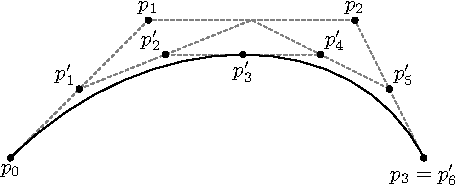
\includegraphics[scale=0.75]{figure/subdivision} \caption{Subdiv. graph}\label{fig:subd}
\end{figure}
Here is a reference to this image: Figure \ref{fig:subd}. Note that \texttt{echo=FALSE} is specified so that the \textbf{R} code is hidden in the document.

\textbf{More Figure Stuff}

Lastly, we will explore how to rotate and enlarge figures using the \texttt{out.extra} chunk option. (Currently this only works in the PDF version of the book.)
\begin{figure}
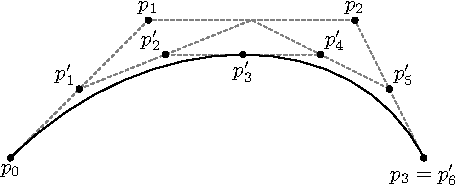
\includegraphics[angle=180, scale=1.1]{figure/subdivision} \caption{A Larger Figure, Flipped Upside Down}\label{fig:subd2}
\end{figure}
As another example, here is a reference: Figure \ref{fig:subd2}.

\hypertarget{footnotes-and-endnotes}{%
\subsection*{Footnotes and Endnotes}\label{footnotes-and-endnotes}}
\addcontentsline{toc}{subsection}{Footnotes and Endnotes}

You might want to footnote something.\footnote{footnote text} The footnote will be in a smaller font and placed appropriately. Endnotes work in much the same way.

\hypertarget{methodology}{%
\chapter*{Methodology}\label{methodology}}
\addcontentsline{toc}{chapter}{Methodology}

The methodology section may include the following subsections:
\begin{itemize}
\tightlist
\item
  Data
\item
  Descriptive analyses
\item
  Modeling Framework
\end{itemize}
\hypertarget{methodology-data}{%
\section*{Data}\label{methodology-data}}
\addcontentsline{toc}{section}{Data}

\textbf{General description of the data and source(s). This includes limitations and delimitations; units of analysis; time window for aggregation and modeling (if applicable); and validation and development samples.}

Let's revisit the work of E.W. Crampton's November 22, 1946 paper titled \emph{The Growth of the Odontoblasts of the Incisor Tooth as a Criterion of the Vitamin C Intake of the Guinea Pig}. It is one of the data sets available within in the R statistical programming environment.

From the description file (\texttt{?ToothGrowth}):
\begin{quote}
The response is the length of odontoblasts (cells responsible for tooth growth) in 60 guinea pigs. Each animal received one of three dose levels of vitamin C (0.5, 1, and 2 mg/day) by one of two delivery methods, orange juice (OJ) or ascorbic acid (a form of vitamin C, coded VC).
\end{quote}
Variables:
\begin{itemize}
\tightlist
\item
  \emph{len}: \emph{numeric}. Tooth length
\item
  \emph{supp}: \emph{factor}. Supplement type (VC or OJ).
\item
  \emph{dose}: \emph{numeric}. Dose in milligrams/day
\end{itemize}
\begin{Shaded}
\begin{Highlighting}[]
\KeywordTok{data}\NormalTok{(ToothGrowth)}
\end{Highlighting}
\end{Shaded}
\hypertarget{methodology-descriptive}{%
\section*{Descriptive analyses}\label{methodology-descriptive}}
\addcontentsline{toc}{section}{Descriptive analyses}

\textbf{Identification of the methodologies that would provide a view into the data. These may include highlighting the relationships that are important for the research, validating assumptions with respect to important metrics, and providing evidence that substantiates the way data is analyzed.}
\begin{Shaded}
\begin{Highlighting}[]
\NormalTok{growth_short <-}\StringTok{ }\KeywordTok{rbind}\NormalTok{(ToothGrowth[}\DecValTok{1}\OperatorTok{:}\DecValTok{7}\NormalTok{,], ToothGrowth[}\DecValTok{26}\OperatorTok{:}\DecValTok{34}\NormalTok{,], ToothGrowth[}\DecValTok{53}\OperatorTok{:}\DecValTok{60}\NormalTok{,])}
\KeywordTok{kable}\NormalTok{(growth_short, }\DataTypeTok{align =} \StringTok{"r"}\NormalTok{, }\DataTypeTok{format =} \StringTok{"latex"}\NormalTok{, }
      \DataTypeTok{longtable =} \OtherTok{TRUE}\NormalTok{, }\DataTypeTok{caption =} \StringTok{"Tooth Growth"}\NormalTok{)}
\end{Highlighting}
\end{Shaded}
\begin{longtable}[t]{l|r|r|r}
\caption{\label{tab:datatable}Tooth Growth}\\
\hline
  & len & supp & dose\\
\hline
1 & 4.2 & VC & 0.5\\
\hline
2 & 11.5 & VC & 0.5\\
\hline
3 & 7.3 & VC & 0.5\\
\hline
4 & 5.8 & VC & 0.5\\
\hline
5 & 6.4 & VC & 0.5\\
\hline
6 & 10.0 & VC & 0.5\\
\hline
7 & 11.2 & VC & 0.5\\
\hline
26 & 32.5 & VC & 2.0\\
\hline
27 & 26.7 & VC & 2.0\\
\hline
28 & 21.5 & VC & 2.0\\
\hline
29 & 23.3 & VC & 2.0\\
\hline
30 & 29.5 & VC & 2.0\\
\hline
31 & 15.2 & OJ & 0.5\\
\hline
32 & 21.5 & OJ & 0.5\\
\hline
33 & 17.6 & OJ & 0.5\\
\hline
34 & 9.7 & OJ & 0.5\\
\hline
53 & 22.4 & OJ & 2.0\\
\hline
54 & 24.5 & OJ & 2.0\\
\hline
55 & 24.8 & OJ & 2.0\\
\hline
56 & 30.9 & OJ & 2.0\\
\hline
57 & 26.4 & OJ & 2.0\\
\hline
58 & 27.3 & OJ & 2.0\\
\hline
59 & 29.4 & OJ & 2.0\\
\hline
60 & 23.0 & OJ & 2.0\\
\hline
\end{longtable}
Table: \ref{tab:datatable}: Head, center, and tail of \emph{Tooth Growth} data.

\newpage

\hypertarget{methodology-modeling}{%
\section*{Modeling Framework}\label{methodology-modeling}}
\addcontentsline{toc}{section}{Modeling Framework}

\textbf{Justification of model(s) selected. Identification of dependent and independent variables, per model as well as variable transformations. Feature extraction (if applicable). Discussion of model(s) functional form. Assumptions of model(s) and ways of insuring that assumptions are observed or tested. Assessing model(s) performance and validation.}

Transform \texttt{dose} into a \texttt{factor}. Only three dosage levels are present.
\begin{Shaded}
\begin{Highlighting}[]
\KeywordTok{data}\NormalTok{(ToothGrowth)}
\KeywordTok{colnames}\NormalTok{(ToothGrowth) <-}\StringTok{ }\KeywordTok{c}\NormalTok{(}\StringTok{"length"}\NormalTok{, }\StringTok{"supplement"}\NormalTok{, }\StringTok{"dose"}\NormalTok{)}
\NormalTok{ToothGrowth}\OperatorTok{$}\NormalTok{dose <-}\StringTok{ }\KeywordTok{as.factor}\NormalTok{(ToothGrowth}\OperatorTok{$}\NormalTok{dose)}
\end{Highlighting}
\end{Shaded}
We are most interested in discovering which treatment leads to the optimal tooth growth.
In this vein, we use \texttt{aggregate} function to transform our data and compute the average tooth \texttt{length} by both \texttt{supplement} type and \texttt{dose} size.
\begin{Shaded}
\begin{Highlighting}[]
\NormalTok{groupedTooth <-}\StringTok{ }\KeywordTok{aggregate}\NormalTok{(ToothGrowth, }\DataTypeTok{by=}\NormalTok{ToothGrowth[,}\DecValTok{2}\OperatorTok{:}\DecValTok{3}\NormalTok{], }\DataTypeTok{FUN=}\NormalTok{mean)[,}\DecValTok{1}\OperatorTok{:}\DecValTok{3}\NormalTok{]}

\KeywordTok{kable}\NormalTok{(groupedTooth, }\DataTypeTok{align =} \StringTok{"r"}\NormalTok{, }\DataTypeTok{caption =} \StringTok{"Average tooth length"}\NormalTok{,}
      \DataTypeTok{format =} \StringTok{"latex"}\NormalTok{, }\DataTypeTok{longtable =} \OtherTok{TRUE}\NormalTok{)}
\end{Highlighting}
\end{Shaded}
\begin{longtable}[t]{r|r|r}
\caption{\label{tab:group}Average tooth length}\\
\hline
supplement & dose & length\\
\hline
OJ & 0.5 & 13.23\\
\hline
VC & 0.5 & 7.98\\
\hline
OJ & 1 & 22.70\\
\hline
VC & 1 & 16.77\\
\hline
OJ & 2 & 26.06\\
\hline
VC & 2 & 26.14\\
\hline
\end{longtable}
\newpage

\hypertarget{math-sci}{%
\section*{Math and Science notation}\label{math-sci}}
\addcontentsline{toc}{section}{Math and Science notation}

\TeX~is the best way to typeset mathematics. Donald Knuth designed \TeX~when he got frustrated at how long it was taking the typesetters to finish his book, which contained a lot of mathematics. One nice feature of \emph{R Markdown} is its ability to read \LaTeX~code directly.

Get around math mode's automatic italicizing in LaTeX by using the argument \texttt{\$\textbackslash{}mathrm\{formula\ here\}\$}, with your formula inside the curly brackets. (Notice the use of the backticks here which enclose text that acts as code.)

So, \(\mathrm{Fe_2^{2+}Cr_2O_4}\) is written \texttt{\$\textbackslash{}mathrm\{Fe\_2\^{}\{2+\}Cr\_2O\_4\}\$}.

The \noindent command below does what you'd expect: it forces the current line/paragraph to not indent. See below and examples of commonly used symbols:

\noindent Exponent or Superscript written as \texttt{\$x\^{}2\$} becomes \(x^2\)

\noindent Subscript written as \texttt{\$x\_1\$} becomes \(x_1\)

\noindent Infinity written as \texttt{\$\textbackslash{}infty\$} becomes \(\infty\)

\noindent alpha written as \texttt{\$\textbackslash{}alpha\$} becomes \(\alpha\)

\noindent beta written as \texttt{\$\textbackslash{}beta\$} becomes \(\beta\)

\noindent delta written as \texttt{\$\textbackslash{}delta\$} becomes \(\delta\)

\noindent epsilon written as \texttt{\$\textbackslash{}epsilon\$} becomes \(\epsilon\)

\noindent sigma written \texttt{\$\textbackslash{}sum\_\{i=1\}\^{}n\ f(x)\$} becomes \(\sum_{i=1}^n f(x)\)

\hypertarget{math-examples}{%
\subsection*{Math Examples}\label{math-examples}}
\addcontentsline{toc}{subsection}{Math Examples}

An Ordinary Least Squares model, from \emph{Introductory Econometrics, 6th edition} by Jeffrey M. Wooldridge, page 27.

\[y_i = \beta_0 + \beta_1 x_i + \epsilon_i\]

An infinite distributed lag (IDL) time series model, by Wooldridge, page 633.

\[ y_t = \alpha + \delta_0 z_t + \delta_1 z_{t-1} + \delta_2 z_{t-2} \ldots + \epsilon_t\]

A vector autoregressive (VAR) model, by Wooldridge, page 657.

\[ y_t = \delta_0 + \alpha_1 y_{t-1} + \gamma_1 z_{t-1} + \alpha_2 y_{t-2} + \gamma_2 z_{t-2} \ldots,\]
\newpage

Determinant of a square matrix:

\[\det\left|\,\begin{matrix}%
c_0&c_1\hfill&c_2\hfill&\ldots&c_n\hfill\cr
c_1&c_2\hfill&c_3\hfill&\ldots&c_{n+1}\hfill\cr
c_2&c_3\hfill&c_4\hfill&\ldots&c_{n+2}\hfill\cr
\,\vdots\hfill&\,\vdots\hfill&
  \,\vdots\hfill&&\,\vdots\hfill\cr
c_n&c_{n+1}\hfill&c_{n+2}\hfill&\ldots&c_{2n}\hfill\cr
\end{matrix}\right|>0\]
\bigskip

A regularization problem solved by Jerome Friedman, Trevor Hastie, Rob Tibshirani and Noah Simon, implemented in the \href{https://cran.r-project.org/web/packages/glmnet/index.html}{R package \texttt{glmnet}}.

\[ \min_{\beta_0,\beta} \frac{1}{N}\sum_{i=1}^N w_il(y_i,\beta_0+\beta^Tx_i)+\lambda \left[(1-\alpha) ||\beta||_2^2/2+\alpha||\beta||_1\right]\]

\bigskip

From Lapidus and Pindar, Numerical Solution of Partial Differential Equations in Science and Engineering, page 54.

\[\int_t\left\{\sum_{j=1}^3 T_j \left({d\phi_j\over dt}+k\phi_j\right)-kT_e\right\}w_i(t)\ dt=0, \qquad\quad i=1,2,3.\]

\bigskip

From Lapidus and Pindar, page 145.

\[\int_{-1}^1\!\int_{-1}^1\!\int_{-1}^1 f\big(\xi,\eta,\zeta\big) = \sum_{k=1}^n\sum_{j=1}^n\sum_{i=1}^n w_i w_j w_k f\big( \xi,\eta,\zeta\big).\]

\hypertarget{additional-r-markdown-and-bookdown-resources}{%
\subsection*{Additional R Markdown and bookdown resources}\label{additional-r-markdown-and-bookdown-resources}}
\addcontentsline{toc}{subsection}{Additional R Markdown and bookdown resources}
\begin{itemize}
\item
  \emph{Bookdown} Online Book - \url{https://bookdown.org/yihui/bookdown/}
\item
  \emph{Markdown} Info Sheet - \url{https://github.com/adam-p/markdown-here/wiki/Markdown-Cheatsheet}
\item
  \emph{R Markdown} Reference Guide - \url{https://www.rstudio.com/wp-content/uploads/2015/03/rmarkdown-reference.pdf}
\end{itemize}
\hypertarget{findings}{%
\chapter*{Findings}\label{findings}}
\addcontentsline{toc}{chapter}{Findings}

Should be organized as follows:
\begin{itemize}
\tightlist
\item
  Results of descriptive analyses
\item
  Modeling results
\item
  Results of model performance and validation
\end{itemize}
\hypertarget{findings-descriptive}{%
\section*{Results of descriptive analyses}\label{findings-descriptive}}
\addcontentsline{toc}{section}{Results of descriptive analyses}
\begin{Shaded}
\begin{Highlighting}[]
\KeywordTok{kable}\NormalTok{(}\KeywordTok{summary}\NormalTok{(ToothGrowth), }\DataTypeTok{align =} \StringTok{"r"}\NormalTok{, }\DataTypeTok{caption =} \StringTok{"Summary of ToothGrowth data"}\NormalTok{,}
      \DataTypeTok{format =} \StringTok{"latex"}\NormalTok{, }\DataTypeTok{longtable =} \OtherTok{TRUE}\NormalTok{)}
\end{Highlighting}
\end{Shaded}
\begin{longtable}[t]{l|r|r|r}
\caption{\label{tab:summary}Summary of ToothGrowth data}\\
\hline
  &     length & supplement &  dose\\
\hline
 & Min.   : 4.20 & OJ:30 & 0.5:20\\
\hline
 & 1st Qu.:13.07 & VC:30 & 1  :20\\
\hline
 & Median :19.25 & NA & 2  :20\\
\hline
 & Mean   :18.81 & NA & NA\\
\hline
 & 3rd Qu.:25.27 & NA & NA\\
\hline
 & Max.   :33.90 & NA & NA\\
\hline
\end{longtable}
Table \ref{tab:summary} above contains summary statistics of the \emph{Tooth Growth} data.

While the code is not displayed to create the graph below (\texttt{echo=FALSE}), it is displayed in the Appendix by referencing the \texttt{boxplot} chunk name..
\begin{figure}
\centering
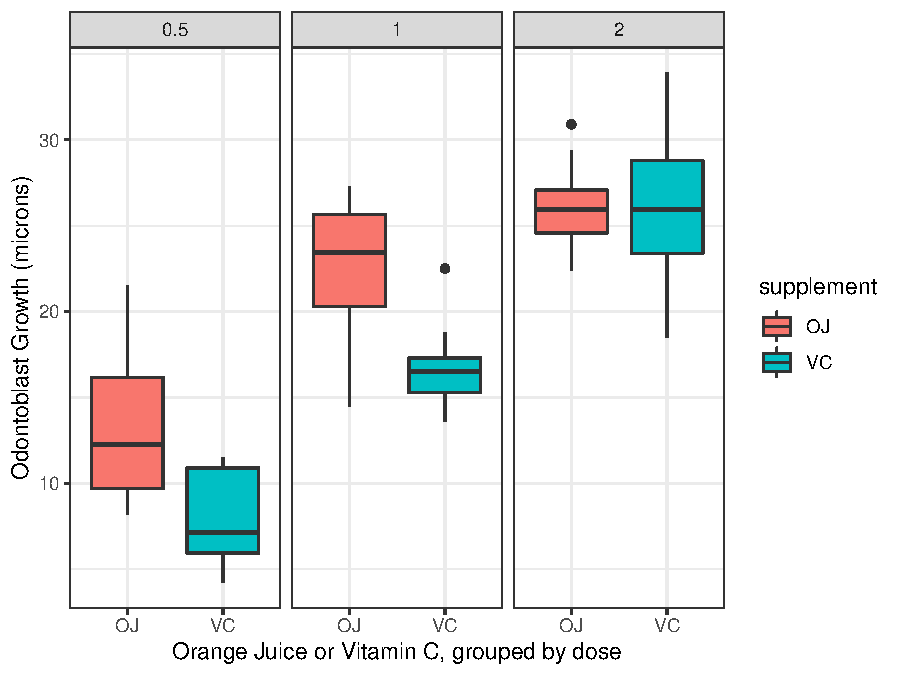
\includegraphics{UChicago-MScA-Capstone_files/figure-latex/boxplot-1.pdf}
\caption{\label{fig:boxplot}Avg. length by supplement and dose}
\end{figure}
Figure \ref{fig:boxplot} was created with the \texttt{ggplot2} package. We can visually compare the average tooth growth by \texttt{supplement} and \texttt{dose}.

\hypertarget{modeling-results}{%
\section*{Modeling results}\label{modeling-results}}
\addcontentsline{toc}{section}{Modeling results}

First, use a \texttt{t.test()} to test \emph{if} dosage leads to growth of incisor length. From the results below, it appears every test rejects the null hypothesis.
\begin{Shaded}
\begin{Highlighting}[]
\NormalTok{test1 <-}\StringTok{ }\KeywordTok{t.test}\NormalTok{(length }\OperatorTok{~}\StringTok{ }\NormalTok{dose, ToothGrowth, dose }\OperatorTok\StringTok{ }\KeywordTok{c}\NormalTok{(}\FloatTok{0.5}\NormalTok{,}\DecValTok{1}\NormalTok{)) }
\NormalTok{test2 <-}\StringTok{ }\KeywordTok{t.test}\NormalTok{(length }\OperatorTok{~}\StringTok{ }\NormalTok{dose, ToothGrowth, dose }\OperatorTok\StringTok{ }\KeywordTok{c}\NormalTok{(}\FloatTok{0.5}\NormalTok{,}\DecValTok{2}\NormalTok{))}
\NormalTok{test3 <-}\StringTok{ }\KeywordTok{t.test}\NormalTok{(length }\OperatorTok{~}\StringTok{ }\NormalTok{dose, ToothGrowth, dose }\OperatorTok\StringTok{ }\KeywordTok{c}\NormalTok{(}\DecValTok{1}\NormalTok{,}\DecValTok{2}\NormalTok{)) }

\NormalTok{testAgg <-}\StringTok{ }\KeywordTok{data.frame}\NormalTok{(}\DataTypeTok{Name =} \KeywordTok{c}\NormalTok{(}\StringTok{"Test 0.5-1"}\NormalTok{, }\StringTok{"Test 0.5-2"}\NormalTok{, }\StringTok{"Test 1-2"}\NormalTok{),}
                  \DataTypeTok{Method =} \KeywordTok{c}\NormalTok{(test1}\OperatorTok{$}\NormalTok{method, test2}\OperatorTok{$}\NormalTok{method, test3}\OperatorTok{$}\NormalTok{method), }
               \DataTypeTok{Pvalue =} \KeywordTok{c}\NormalTok{(test1}\OperatorTok{$}\NormalTok{p.value, test2}\OperatorTok{$}\NormalTok{p.value, test3}\OperatorTok{$}\NormalTok{p.value), }
          \DataTypeTok{Tstat =} \KeywordTok{c}\NormalTok{(test1}\OperatorTok{$}\NormalTok{statistic, test2}\OperatorTok{$}\NormalTok{statistic, test3}\OperatorTok{$}\NormalTok{statistic))}

\KeywordTok{kable}\NormalTok{(testAgg, }\DataTypeTok{digit =} \DecValTok{7}\NormalTok{, }\DataTypeTok{align =} \StringTok{"r"}\NormalTok{, }\DataTypeTok{caption =} \StringTok{"t-test results"}\NormalTok{, }
      \DataTypeTok{format =} \StringTok{"latex"}\NormalTok{, }\DataTypeTok{longtable =} \OtherTok{TRUE}\NormalTok{)}
\end{Highlighting}
\end{Shaded}
\begin{longtable}[t]{r|r|r|r}
\caption{\label{tab:t-test}t-test results}\\
\hline
Name & Method & Pvalue & Tstat\\
\hline
Test 0.5-1 & Welch Two Sample t-test & 1.00e-07 & -6.476648\\
\hline
Test 0.5-2 & Welch Two Sample t-test & 0.00e+00 & -11.799046\\
\hline
Test 1-2 & Welch Two Sample t-test & 1.91e-05 & -4.900484\\
\hline
\end{longtable}
Table \ref{tab:t-test}

\hypertarget{results-of-model-performance-and-validation}{%
\section*{Results of model performance and validation}\label{results-of-model-performance-and-validation}}
\addcontentsline{toc}{section}{Results of model performance and validation}

Next, subset the \texttt{ToothGrowth} data into seperate data sets defined by supplement dose of 0.5, 1, and 2 mg. This allow us to controlling for dose increases of \emph{economic} significance.

Subset tooth data into a separate \texttt{data.frame} for each dosage level. Then Execute the \texttt{t.test()} function for the dosage of 0.5 mg and display the results.
\begin{Shaded}
\begin{Highlighting}[]
\NormalTok{dose05 <-}\StringTok{ }\NormalTok{ToothGrowth[ToothGrowth}\OperatorTok{$}\NormalTok{dose }\OperatorTok{==}\StringTok{ }\FloatTok{0.5}\NormalTok{, ] }
\NormalTok{ dose1 <-}\StringTok{ }\NormalTok{ToothGrowth[ToothGrowth}\OperatorTok{$}\NormalTok{dose }\OperatorTok{==}\StringTok{ }\DecValTok{1}\NormalTok{, ]}
\NormalTok{ dose2 <-}\StringTok{ }\NormalTok{ToothGrowth[ToothGrowth}\OperatorTok{$}\NormalTok{dose }\OperatorTok{==}\StringTok{ }\DecValTok{2}\NormalTok{, ]}

\NormalTok{ test4 <-}\StringTok{ }\KeywordTok{t.test}\NormalTok{(length }\OperatorTok{~}\StringTok{ }\NormalTok{supplement, }\DataTypeTok{data =}\NormalTok{ dose05)}
\NormalTok{ test5 <-}\StringTok{ }\KeywordTok{t.test}\NormalTok{(length }\OperatorTok{~}\StringTok{ }\NormalTok{supplement, }\DataTypeTok{data =}\NormalTok{ dose1)}
\NormalTok{ test6 <-}\StringTok{ }\KeywordTok{t.test}\NormalTok{(length }\OperatorTok{~}\StringTok{ }\NormalTok{supplement, }\DataTypeTok{data =}\NormalTok{ dose2)}
\end{Highlighting}
\end{Shaded}
Place the results of the analysis directly into your content with \textbf{\emph{inline code}} functions:

With a very low p-value of 0.0064 and a corresponding t-statistic of 3.1697, it appears that at low doses, \emph{Orange Juice} is the preferable delivery mechanism to \emph{Vitamin C} for Ascorbic Acid delivery.

The p-value and t-statistic above have been directly extracted from the model object and printed inline. using the `r foo' syntax with quotes(') replaced by back-ticks (`).

\hypertarget{conclusion}{%
\chapter*{Conclusion}\label{conclusion}}
\addcontentsline{toc}{chapter}{Conclusion}

This section includes a concise summary of the findings. Your summary might be organized by the research objectives or hypotheses. Make sure you address the extent to which research objectives are achieved, and if they are not achieved, explain why. Make sure to interpret your findings in a way that acknowledges the limitations of the research. That is, do not extrapolate the insights derived from your research to situations you have not examined.

\emph{While increasing dosage leads to larger incisor length, the choice of delivery mechanism between Orange Juice and Vitamin C does not seem to make a difference. However, at very low levels, Orange Juice appears more effective, displaying higher average growth.}

\hypertarget{recommendations}{%
\chapter*{Recommendations}\label{recommendations}}
\addcontentsline{toc}{chapter}{Recommendations}

Includes guidelines as to ways in which your results should or could be used in practice. You may discuss other uses of your results, if there are any. The ways to extend your analysis and the benefits of doing so might be included in this section as well.

\appendix

\hypertarget{the-first-appendix}{%
\chapter{The First Appendix}\label{the-first-appendix}}

This first appendix includes all of the R chunks of code that were hidden throughout the document (using the \texttt{include\ =\ FALSE} chunk tag) to help with readibility and/or setup.

\textbf{In section} \ref{pressure-plot}:
\begin{Shaded}
\begin{Highlighting}[]
\KeywordTok{plot}\NormalTok{(pressure, }\DataTypeTok{type =} \StringTok{"l"}\NormalTok{, }\DataTypeTok{col=}\StringTok{"cornflowerblue"}\NormalTok{, }\DataTypeTok{lwd =} \DecValTok{2}\NormalTok{,}
               \DataTypeTok{xlab =} \StringTok{"Temperature (deg C)"}\NormalTok{,}
               \DataTypeTok{ylab =} \StringTok{"Pressure (mm of Hg)"}\NormalTok{,}
               \DataTypeTok{main =} \StringTok{"pressure data: Vapor Pressure of Mercury"}\NormalTok{,}
               \DataTypeTok{frame =} \OtherTok{FALSE}\NormalTok{)}
\end{Highlighting}
\end{Shaded}
\textbf{In section \ref{ref-labels}:}
\begin{Shaded}
\begin{Highlighting}[]
\KeywordTok{data}\NormalTok{(ToothGrowth)}
\KeywordTok{colnames}\NormalTok{(ToothGrowth) <-}\StringTok{ }\KeywordTok{c}\NormalTok{(}\StringTok{"length"}\NormalTok{, }\StringTok{"supplement"}\NormalTok{, }\StringTok{"dose"}\NormalTok{)}
\NormalTok{ToothGrowth}\OperatorTok{$}\NormalTok{dose <-}\StringTok{ }\KeywordTok{as.factor}\NormalTok{(ToothGrowth}\OperatorTok{$}\NormalTok{dose)}

\NormalTok{groupedTooth <-}\StringTok{ }\KeywordTok{aggregate}\NormalTok{(ToothGrowth, }\DataTypeTok{by=}\NormalTok{ToothGrowth[,}\DecValTok{2}\OperatorTok{:}\DecValTok{3}\NormalTok{], }\DataTypeTok{FUN=}\NormalTok{mean)[,}\DecValTok{1}\OperatorTok{:}\DecValTok{3}\NormalTok{]}

\KeywordTok{library}\NormalTok{(ggplot2)}
 \KeywordTok{ggplot}\NormalTok{(ToothGrowth, }\KeywordTok{aes}\NormalTok{(}\DataTypeTok{x =}\NormalTok{ supplement, }\DataTypeTok{y =}\NormalTok{ length)) }\OperatorTok{+}\StringTok{ }
\StringTok{                     }\KeywordTok{geom_boxplot}\NormalTok{(}\KeywordTok{aes}\NormalTok{(}\DataTypeTok{fill=}\NormalTok{supplement)) }\OperatorTok{+}\StringTok{ }
\StringTok{                     }\KeywordTok{facet_wrap}\NormalTok{(}\OperatorTok{~}\NormalTok{dose) }\OperatorTok{+}\StringTok{ }
\StringTok{                     }\KeywordTok{guides}\NormalTok{(}\DataTypeTok{colour =} \KeywordTok{guide_legend}\NormalTok{(}\StringTok{"Color = Supplement"}\NormalTok{)) }\OperatorTok{+}\StringTok{ }
\StringTok{                     }\KeywordTok{labs}\NormalTok{(}\DataTypeTok{x=}\StringTok{"Orange Juice or Vitamin C, grouped by dose"}\NormalTok{, }
                          \DataTypeTok{y=}\StringTok{"Odontoblast Growth (microns)"}\NormalTok{)  }\OperatorTok{+}
\StringTok{                     }\KeywordTok{theme_bw}\NormalTok{()}
\end{Highlighting}
\end{Shaded}
\hypertarget{a-second-appendix-for-example}{%
\chapter{A Second Appendix, for example}\label{a-second-appendix-for-example}}

\backmatter

\hypertarget{references}{%
\chapter*{References}\label{references}}
\addcontentsline{toc}{chapter}{References}

\markboth{References}{References}

\noindent

\setlength{\parindent}{-0.20in}
\setlength{\leftskip}{0.20in}
\setlength{\parskip}{8pt}

There are a variety of tools available for creating a bibliography database (stored with the .bib extension). In addition to BibTeX suggested below, you may want to consider using the free and easy-to-use tool called \href{https://www.zotero.org/}{Zotero}.

\emph{R Markdown} uses \emph{pandoc} (\url{http://pandoc.org/}) to build its bibliographies. To cite references in your thesis (after creating your bibliography database), place the reference name inside square brackets and precede it by the ``at'' symbol. For example, here's a reference to a book about worrying: (Molina \& Borkovec, 1994). This \texttt{Molina1994} entry appears in a file called \texttt{thesis.bib} in the \texttt{bib} folder. This bibliography database file was created by a program called BibTeX. You can call this file something else if you like (look at the YAML header in the main .Rmd file) and, by default, is to placed in the \texttt{bib} folder.

\textbf{Additional Tips}
\begin{itemize}
\tightlist
\item
  The sooner you start compiling your bibliography for something as large as a capstone, the better. Typing in source after source is mind-numbing enough; do you really want to do it for hours on end at the last minute?
\item
  The cite key (a citation's label) needs to be unique from the other entries.
\item
  When you have more than one author or editor, you need to separate each author's name by the word ``and'' e.g. \texttt{Author\ =\ \{Noble,\ Sam\ and\ Youngberg,\ Jessica\},}
\end{itemize}
\textbf{Example output generated from bib file}

\hypertarget{refs}{}
\leavevmode\hypertarget{ref-angel2000}{}%
Angel, E. (2000). \emph{Interactive computer graphics : A top-down approach with opengl}. Boston, MA: Addison Wesley Longman.

\leavevmode\hypertarget{ref-angel2001}{}%
Angel, E. (2001a). \emph{Batch-file computer graphics : A bottom-up approach with quicktime}. Boston, MA: Wesley Addison Longman.

\leavevmode\hypertarget{ref-angel2002a}{}%
Angel, E. (2001b). \emph{Test second book by angel}. Boston, MA: Wesley Addison Longman.

\leavevmode\hypertarget{ref-Molina1994}{}%
Molina, S. T., \& Borkovec, T. D. (1994). The Penn State worry questionnaire: Psychometric properties and associated characteristics. In G. C. L. Davey \& F. Tallis (Eds.), \emph{Worrying: Perspectives on theory, assessment and treatment} (pp. 265--283). New York: Wiley.


% Index?

\end{document}
